\documentclass[12pt]{article}

% Package lists
\usepackage{pythonhighlight}
\usepackage{solarized-dark}
\usepackage{geometry}
\usepackage{graphicx}

% Configurations
\geometry{margin=1cm, bottom=2cm}
\setlength{\columnseprule}{1pt}

\begin{document}
  \title{Report Lab 5}
  \author{Nguyen Tien Duc - ITITIU18029}
  \maketitle
  \part*{1/ Golden-Section Search}
    \section*{Code}
      \inputpython{../GoldenSectionSearch.py}{0}{35}
    \section*{Running}
    \begin{center}
      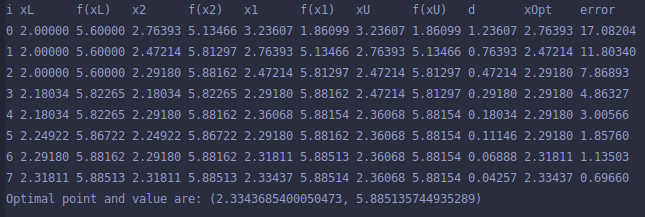
\includegraphics{../GoldenSectionSearch.png}
    \end{center}
  \part*{2/ Random Search, Grid Search and AutoML(Bayesian Optimization)}
    \section*{Code}
      \subsection*{Random vs Grid Search}
      \inputpython{../RandomVsGrid.py}{0}{98}
      \subsection*{Bayesian Optimization using bayes-opt}
      \inputpython{../Bayesian.py}{0}{19}
    \section*{Running}
      \subsection*{Random vs Grid 100 steps}
        \begin{center}
          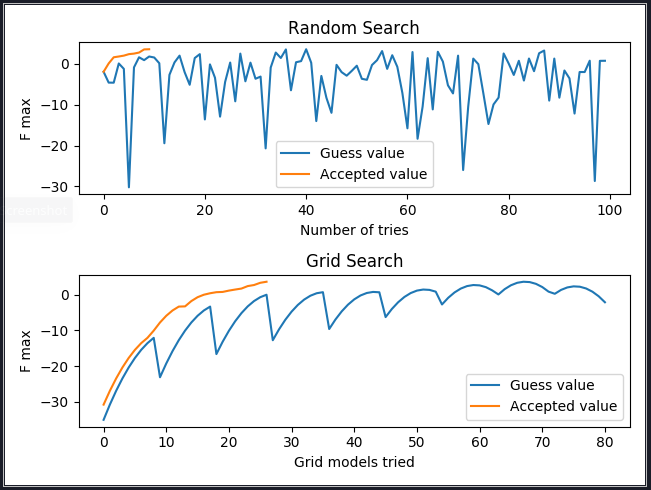
\includegraphics{../RandomVsGrid100Plot.png}
          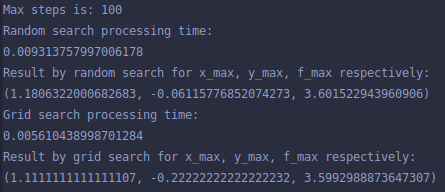
\includegraphics{../RandomVsGrid100Result.png}
        \end{center}
      \subsection*{Random vs Grid 400 steps}
        \begin{center}
          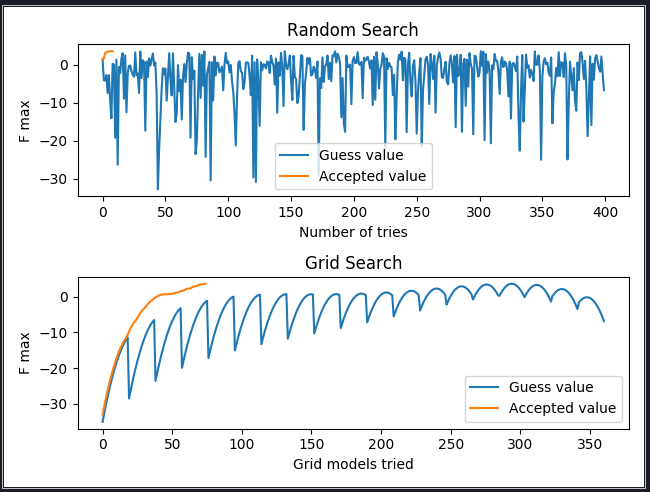
\includegraphics{../RandomVsGrid400Plot.png}
          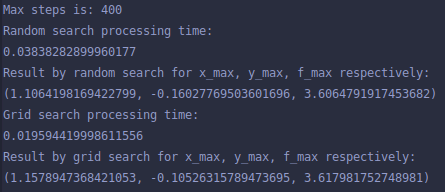
\includegraphics{../RandomVsGrid400Result.png}
        \end{center}
      \subsection*{Random vs Grid 900 steps}
        \begin{center}
          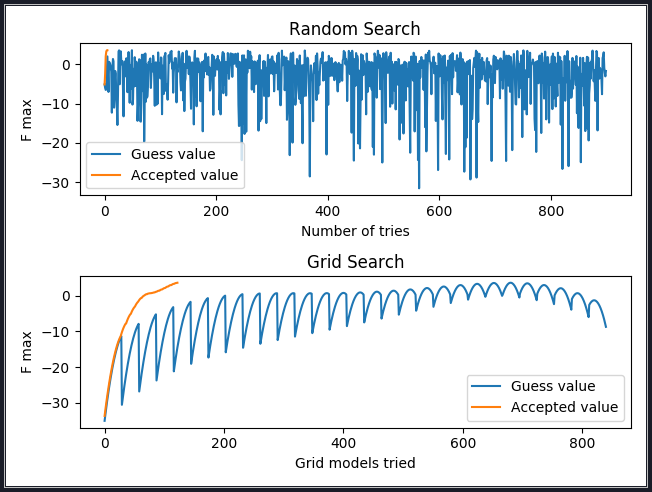
\includegraphics{../RandomVsGrid900Plot.png}
          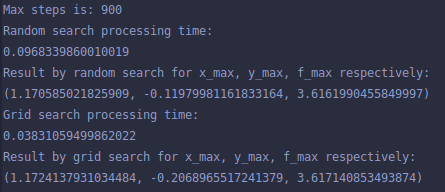
\includegraphics{../RandomVsGrid900Result.png}
        \end{center}
      \subsection*{Bayesian 20 steps}
        \begin{center}
          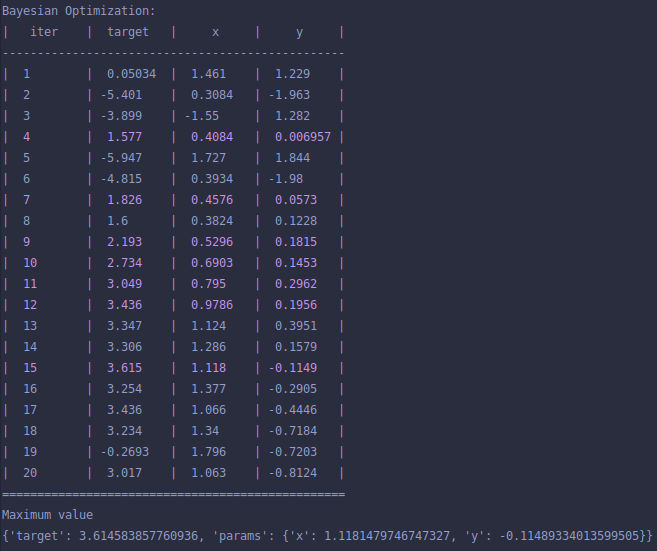
\includegraphics{../BayesianResult.png}
        \end{center}
  \part*{Analysis and Comparison}
    Firstly, this test and comparison between grid search, random search and bayesian Optimization is nowhere perfect.
    Obvious flops are:
      \begin{itemize}
        \item Only one function is used for all tests.
        \item Test object(the function) is too simple to demonstrate the methods.
        \item Bayesian implementation is borrowed from external source. Thus, it is not thoroughly understood.
      \end{itemize}
    \section*{Random Search vs Grid Search}
    The result from 3 different numbers of maximum steps clearly show that random search is more efficient as an algorithm.\\
    In all 3 cases, random search always takes longer to process all the steps but, however, always takes less steps to reach the optimal point than grid search. \\
    \(\Rightarrow\) The long processing time of random search is substituted by a much faster approach to the solution.

      \begin{center}
        \begin{tabular}{||c||c|c||} 
        \hline \hline
        & Random Search & Grid Search \\
        \hline
        Max Time & Longer, depends on Random algorithm & Faster as linspace algorithm is has linear time \\ 
        Solve Time & Faster, independent of max steps & Longer, depends on max steps to form the grids \\ 
        Accuracy & Unpredictable, but performs better in 3 cases & Predictable, but performs worse in 3 cases\\
        \hline \hline
        \end{tabular}
      \end{center}
    \section*{AutoML(Bayesian) vs Non-AutoML(Random/Grid)}
    From the Bayesian data, it takes 15 iterations to reach the solution, not an impressive performance.\\
    However, this result depends on the implementation of Bayesian Optimization from bayes-opt package.\\
    In theory, Bayesian, as an auto-machine-learning method, proved to be really efficient as new choices are sampled from the data based on the history probability, thus able to avoid bad patterns and reach the optimization solution faster.
      \begin{center}
        \begin{tabular}{||c||c|c||} 
        \hline \hline
        & AutoML(Bayesian) & Non-AutoML(Random/Grid) \\
        \hline
        Max Time & Longer, depends on bayes-opt algorithm & Faster as algorithm is customized for this test \\ 
        Solve Time & Good but not impressive, same as Random & Grid search is still the longest \\ 
        Accuracy & Bad guesses are corrected immediately & Either unpredictable or ill-performed \\
        \hline \hline
        \end{tabular}
      \end{center}
    \section*{Conclusion}
      \begin{itemize}
        \item Between the naive, non-machine-learning, methods, random search is the obvious best. Grid search is too tedious, as every models is tested for optimization, this will be a burden if the object function is too costly to compute.
        \item However, even with the better random search method, as the function becomes harder to compute and the variables bounds get complicated (e.g. becomes piece-wise), it will be really costly to regenerate random samples, and, costly to evaluate random, meaningless samples. 
        \item As a result, between the best candidate of naive methods and auto-machine-learning methods, i.e. random search vs bayesian optimization, AutoML still proved to be a bester choice because only methods from AutoML that can learn from the past statistics is capable of optimizing real world problems, which is usually complicated, messy, non-linear, multidimensional, ...
        \item Finally, we can rank the 3 methods above as: Bayesian Optimization \(>\) Random search \(>\) Grid search
      \end{itemize}

\end{document}